% Anonymous main-text compression, 2026-10-08. Complete evidence is retained
% in the existing supplementary project. No new inference or journal reads.
\begin{abstract}
Evaluating a workflow produces quality information and reusable execution
state, changing the cost of later evaluations. AgentUCT adds an economic
model of execution to UCT: saved prefixes, observed bills and continuation
demand estimate the remaining cost of obtaining a complete quality observation.
That price guides allocation while raw quality is backed up. We characterize
the execution information sufficient for exact completion pricing and prove
logarithmic cumulative training-quality regret on finite trees with fixed
scores, bounded cold prices and persistent successful execution.
In a shared HotpotQA RAG system, AgentUCT achieves $69.57\pm0.28\%$ test F1
at a 32M weighted-token search budget, compared with $68.01\pm1.12\%$ for
MCTS-UCT over five paired seeds. The advantage persists when the training-best
workflow is tested without validation. AgentUCT has the highest 32M mean
among eleven methods in this protocol, with seed-level and smaller-budget
exceptions. On GSM8K, its largest-budget mean is slightly higher than MCTS-UCT
and equal to AFlow. Completion pricing improves allocation in the tested
RAG regime; neither the theory nor the generated-workflow results establish
universal finite-budget superiority.
\end{abstract}
\ifdefined\AgentUCTAAMAS
\maketitle
\fi

\section{Introduction}
An agent optimizing a discrete workflow needs an economic model of its own
experiments. A quality observation can require several language-model calls
and retrieval steps. Workflows share executable prefixes, so evaluating one
changes the remaining cost of evaluating others. Under a fixed search budget,
the question is how to use that changing execution state to discover a
high-quality workflow while preserving quality exploration.

UCT allocates evaluations using backed-up quality and an exploration
bonus~\citep{kocsis2006bandit}. Its index stays unchanged when saved work
changes but quality and visit counts remain fixed. A common cache can reduce
execution cost without making allocation responsive to that cost.
Pipeline optimizers already exploit reusable intermediates
\citep{zhang2016flash,essofi2024memoization,torresi2026multistage}.
The issue for tree search is the cost horizon: a cheap or cached first step
can still precede an expensive suffix needed to obtain quality feedback.

AgentUCT separates the workflow tree from a bipartite query--prefix execution
graph. It subtracts the predicted remaining bill of a complete observation
from UCT's quality-and-exploration index. Saved states identify reusable work,
physical receipts estimate missing-work prices, and a continuation model
predicts the work demanded by a branch. Complete feedback updates the model
and raw-return tree statistics before the next decision. Historical charges
do not become permanent deductions from a workflow's quality.

We test this intervention against MCTS-UCT with shared initialization,
expansion, rollout and execution settings in HotpotQA. First-unpaid and static
complete-cost ablations test the estimator's horizon and adaptation; direct
training-Top1 testing examines dependence on validation. Editing, sampling
and surrogate controls extend competition within the same grammar. The complete
five-seed GSM8K comparison measures transfer to generated programs. The theory characterizes sufficient execution information,
a same-state cost exchange, and quality exploration under persistent finite
execution. Its completed-evaluation guarantee and the measured finite-budget
test outcomes answer separate questions.

\section{Execution State and Cost-Aware Tree Search}
\label{sec:setting}
\subsection{A search tree and a cache graph}
Let $\mathcal X$ be a finite nonempty prefix-antichain of terminal workflows.
Their legal prefixes form a tree $\mathcal T$, rooted at $\varnothing$.
Write $pa$ for prefix $p$ extended by action $a$, and $\mathcal X(pa)$ for
its terminal descendants. With query universe $\mathcal U$, active nonempty
panel $\mathcal Q$ and full execution prefixes $\mathcal P$, the saved state is
\begin{equation}
G_t=(\mathcal U,\mathcal P,K_t),\qquad K_t\subseteq\mathcal U\times\mathcal P.
\label{eq:graph}
\end{equation}
An edge $(q,u)$ identifies a restorable object for input $q$ after prefix $u$
in the current namespace. Tree edges specify legal decisions; execution edges
identify saved work. A state saved for one input cannot replace another's.

Let $\mathcal D(x)$ be the query--prefix resources demanded by terminal $x$,
including any fixed execution prefix, with nonnegative weights $w_r$.
For persistent, prefix-complete publication,
\begin{equation}
b_t^{\mathrm{cold}}(x)=\sum_{r\in\mathcal D(x)\setminus K_t}w_r,
\qquad K_{t+1}=K_t\cup\mathcal D(x_t).
\label{eq:cold}
\end{equation}
This is each query's suffix after its deepest saved checkpoint. Empty
initialization and publication of every successful intermediate preserve
prefix completeness. Sparse checkpoints require the suffix definition
directly; eviction or failed publication requires a different model.
Nonreusable work $h_t(x)\ge0$ gives the full physical bill
\begin{equation}
b_t(x)=b_t^{\mathrm{cold}}(x)+h_t(x).
\label{eq:bill}
\end{equation}
Repeated proposal and repair calls remain charged when actually incurred.
Prices use one declared unit; tokens and wall time are reported separately.

\begin{figure*}[t]
\centering
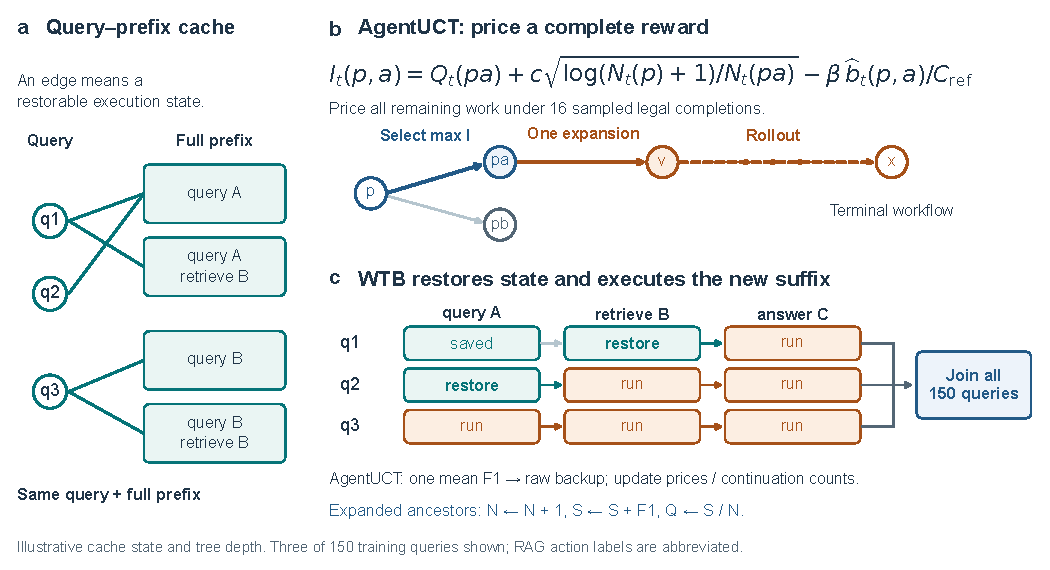
\includegraphics[width=\textwidth]{figures/agentuct-overview-20261004/agentuct-overview.pdf}
\caption{AgentUCT separates execution state, allocation and physical evaluation.
(a) Query--prefix edges identify restorable states. (b) Raw-return means,
exploration and predicted complete-observation cost select a branch;
expansion inserts one child. (c) Execution restores each input's deepest
checkpoint and runs its missing suffix. All training inputs join before one
raw-quality backup and the next price update. Rollout prefixes may be saved
without receiving tree statistics. The illustration describes the general
mechanism; the RAG experiment uses full-panel publication and its adaptive
selections occurred at the root.}
\Description{Saved query-prefix states inform a cost-aware tree selector. A selected workflow restores input-specific checkpoints, executes missing steps, and joins all outcomes before updating raw quality and observed execution prices.}
\label{fig:agentuct-overview}
\end{figure*}

\subsection{Allocation and complete feedback}
The main theorem fixes $f:\mathcal X\to[0,1]$, a full-panel score table.
Each event expands at most one node $v_t$ and completes a terminal $x_t$
extending it. For every expanded ancestor $p\preceq v_t$,
\begin{equation}
\begin{aligned}
N_{t+1}(p)&=N_t(p)+1,\\
S_{t+1}(p)&=S_t(p)+f(x_t),\qquad Q_t(p)=S_t(p)/N_t(p).
\end{aligned}
\label{eq:backup}
\end{equation}
Rollout can publish deeper execution prefixes without inserting their tree
nodes. A cached-terminal replay is another backed-up return, not an
independent model sample. Incomplete panels receive no backup and fall
outside the successful-completion theorem. Empirical candidate errors that
return a score remain scored and billed.

Unvisited legal children are taken first. Among initialized children,
AgentUCT maximizes
\begin{equation}
I_t(p,a)=Q_t(pa)+c\sqrt{\frac{\log(N_t(p)+1)}{N_t(pa)}}
-\gamma\widehat b_t(p,a),\qquad\gamma=\beta/C_{\rm ref}.
\label{eq:index}
\end{equation}
Here $c>0$, $\beta\ge0$ and $C_{\rm ref}>0$. Costs condition on pre-decision
state; raw quality remains the reward signal. MCTS-UCT sets $\beta=0$ while
retaining the same execution cache service.

\begin{algorithm}[t]
\caption{AgentUCT with complete feedback and actual-cost snapshots}
\label{alg:agentuct}
\begin{algorithmic}[1]
\Require Legal workflows, panel, cache, estimator, $c,\beta,C_{\rm ref}$
\State Initialize root statistics and actual-cost ledger
\While{the evaluation safety horizon has not been reached}
\State Traverse initialized nodes using~\eqref{eq:index}
\State Expand one unvisited legal child, when available
\State Complete a terminal by the declared rollout rule
\State Restore checkpoints and finish the whole training panel
\State Record all physical receipts; publish successful objects
\If{the complete panel returns a score}
\State Update cost observations and continuation counts
\State Back up raw quality through expanded ancestors
\State Save tree, cache and cumulative actual-cost snapshot
\EndIf
\If{actual search cost reaches the largest reporting budget}
\State \textbf{break}
\EndIf
\EndWhile
\State Retain the last complete affordable snapshot per budget
\State Select an endpoint by the declared held-out protocol
\end{algorithmic}
\end{algorithm}

\section{The Cost of Obtaining a Complete Reward}
\label{sec:estimation}
The target is the remaining bill conditional on history and the chosen child,
\begin{equation}
m_t(p,a)=\E_{\rho_{\mathrm{exec},t}}[b_t(X)\mid p,a].
\label{eq:actualmean}
\end{equation}
It covers the complete reward-producing suffix. Current cache membership is
observed; missing-resource prices and future demand are predicted. A declared
reference continuation law gives the cold estimate
\begin{equation}
\widehat b_t^{\mathrm{cold}}(p,a)=
\sum_{x\in\mathcal X(pa)}\rho_{C,t}(x\mid p,a)
\sum_{r\in\mathcal D(x)\setminus K_t}\widehat w_{t,r}.
\label{eq:reference}
\end{equation}
The law is normalized on legal terminals and may differ from actual
continuation. Forecast weights satisfy $0\le\widehat w_{t,r}\le M_r$ for
a fixed finite envelope. Prediction bounds clip forecasts, not physical
charges or admission of evaluations.

For a resource ending in action $a$, online prices combine a calibrated
pseudo-observation $\mu_a^0$ and observed physical costs $c_i$:
\begin{equation}
\widehat\mu_{t,r}=\frac{\mu_a^0+\sum_{i\in I_t(r)}\min\{c_i,M_a\}}
{1+|I_t(r)|},\qquad 0\le\mu_a^0\le M_a.
\label{eq:online-mean}
\end{equation}
The observation pool uses qid--prefix data when available, then prefix data
across queries, then action data across prefixes. Physical hits supply no
new cost observation; known zero-work slots have zero forecast price.

If $n_t(p,a)$ counts complete training paths taking $a$ after $p$, the
historical next-action law is
$(n_t(p,a)+1/|A(p)|)/(\sum_b n_t(p,b)+1)$.
Uniform-complete instead uses $1/|A(p)|$. With $d_q(x,K_t)$ the deepest
saved prefix depth, $m=16$ sampled legal completions estimate
\begin{equation}
\widehat b_t^{\mathrm{cold}}(p,a)=\frac1m\sum_{i=1}^m
\sum_{q\in\mathcal Q}\sum_{d_q(X_i,K_t)<j\le|X_i|}
\widehat w_{t,(q,X_{i,1:j})}.
\label{eq:sample-cost}
\end{equation}
Multiplicity is retained. Pricing freezes cache, means and counts and makes
no model calls or exhaustive subtree traversal. Equivalently, with reference
demand probability $\pi_{t,r}$,
\begin{equation}
\widehat b_t^{\mathrm{cold}}(p,a)=\sum_r\pi_{t,r}(p,a)\widehat w_{t,r}.
\label{eq:resourceform}
\end{equation}
Linearity needs no independence among resources. Resource-price, continuation
and sampling errors remain; changing those models can increase a forecast
even as the cache grows. This one-observation estimate does not value a
multi-step investment in future saved work.

AgentUCT-NextC retains only the first positive unpaid resource per query.
If its position on completion $X$ is $j_t(q,X)$, with price zero when none exists,
\begin{equation}
\widehat b_t^{\mathrm{unpaid}}(p,a)=
\E_{X\sim\rho_{C,t}}\sum_{q\in\mathcal Q}
\widehat w_{t,(q,X_{1:j_t(q,X)})}.
\label{eq:next-unpaid}
\end{equation}
It is bounded by the complete cold estimate on the same sampled paths and
isolates the omitted suffix. An immediate-child estimate differs: an
initialized child's prefix is already saved under persistent full-panel
publication, making its direct cold penalty zero.

\section{Which Cache Information Changes Allocation?}
\label{sec:graph-information}
The allowed query demands determine the cost information a search must retain.
A cache is sufficient for restoration only when the compatible execution objects
are available. For pricing, several queries can sometimes be aggregated.

\begin{theorem}[Demand-profile quotient]
\label{thm:demand-quotient}
Fix the family of allowed panels $\mathcal Q_1,\ldots,\mathcal Q_m$.
Group queries by their membership profiles
$q\sim r$ if $\ind\{q\in\mathcal Q_j\}=\ind\{r\in\mathcal Q_j\}$ for every $j$.
For each group $C$ and prefix $u$, store
\begin{equation}
 R_K(C,u)=\sum_{q\in C}\ind\{(q,u)\notin K\}w_{q,u}.
 \label{eq:group-residual}
\end{equation}
The bill for an allowed demand $\mathcal Q_j\times P_x$ equals
\[
 \sum_{u\in P_x}\sum_{C\subseteq\mathcal Q_j}R_K(C,u).
\]
Publishing that demand sets precisely these group--prefix cells to zero.
Conversely, merging two queries that some allowed panel separates loses the
ability to recover every panel bill from group residual sums, already with
unit weights and arbitrary binary residual states.
\end{theorem}

\paragraph{Proof.}
Every allowed panel contains either all or none of a profile group. Partitioning
the query sum therefore gives its exact bill, and publication removes precisely
the demanded cells. For the converse, swap one unit of uncached demand between
two merged queries. The group total stays fixed, while a separating panel's bill
changes. A common summary cannot recover both bills. Lean checks both directions.

\begin{proposition}[Full-panel compression]
\label{prop:graph-compression}
Fix the panel $\mathcal Q$ and resource weights. For an arbitrary cache $K$, define the residual prefix bill
\begin{equation}
 r_K(u)=\sum_{q\in\mathcal Q}\ind\{(q,u)\notin K\}w_{q,u}.
 \label{eq:residual-prefix}
\end{equation}
For a full-panel demand $\mathcal Q\times P_x$, its cold bill is $\sum_{u\in P_x}r_K(u)$. Publishing this demand sets $r_K(u)$ to zero on $P_x$ and leaves the other residual bills unchanged. If $K=\mathcal Q\times S$, the bill further reduces to $\sum_{u\in P_x\setminus S}\bar w_u$, where $\bar w_u=\sum_qw_{q,u}$. Empty initialization followed by full-panel publication preserves this rectangular form.
\end{proposition}

The main experiment uses this fixed-full-panel case. Its completion bills admit
an exact prefix-level quotient. The qid--prefix model also specifies the physical
checkpoints and the query-conditioned price observations; these are separate
from the aggregated cost totals. Online price revisions refresh the residual
sums, as detailed in the supplementary material.

Selective demands can require finer information. Consider two queries, prefixes
$u,v$, unit prices, and the caches
\[
 K_1=\{(q_0,u),(q_1,v)\},\quad
 K_2=\{(q_1,u),(q_0,v)\}.
\]
Both prefixes have one full-panel residual unit in either state.
On query $q_0$, their bills are $(0,1)$ and $(1,0)$. Equal-quality allocation
therefore reverses. The supplement gives a separation reachable from empty
caches through complete overlapping-panel evaluations. The result identifies
necessary information within partition-based residual summaries; bitsets and
other lossless encodings can preserve that same information.

\section{Why Price Complete Evaluations?}
\label{sec:finite-budget}
At a common tree and cache state, let $U_a$ be ordinary UCT's quality index.
Complete prices allow a precise exchange between that index and evaluation cost:
\begin{equation}
 U_a-\gamma b_a\ge U_b-\gamma b_b
 \quad\Longleftrightarrow\quad
 U_b-U_a\le\gamma(b_b-b_a).
 \label{eq:completion-threshold}
\end{equation}

\begin{proposition}[What pricing buys at the current state]
\label{prop:priced-tradeoff}
Let $b$ maximize ordinary UCT's $U$, and let $a$ maximize
$U-\gamma\widehat b$ over the same initialized candidates, with $\gamma>0$.
Then
\begin{equation}
 \widehat b_a\le\widehat b_b,\qquad
 0\le U_b-U_a\le\gamma(\widehat b_b-\widehat b_a).
 \label{eq:priced-tradeoff}
\end{equation}
If $|\widehat b_j-b_j|\le\epsilon_j$ for $j=a,b$, the actual expected saving obeys
\begin{equation}
 b_b-b_a\ge\widehat b_b-\widehat b_a-\epsilon_a-\epsilon_b.
 \label{eq:physical-saving}
\end{equation}
\end{proposition}

\paragraph{Proof.}
Ordinary-UCT maximality gives $U_b\ge U_a$; priced maximality gives
$U_b-U_a\le\gamma(\widehat b_b-\widehat b_a)$. Nonnegative quality sacrifice
implies predicted cost savings. The two cost-error bounds give the physical
saving inequality. A predicted saving exceeding their sum certifies cheaper
expected execution.

The bill must cover the complete reward-producing suffix. If two candidates
have the same immediate-edge cost, a direct-edge penalty cannot distinguish
their tails. The full rule changes the choice when the tail saving exceeds the
quality-index difference divided by $\gamma$. For persistent full-panel caches,
an initialized direct child is already saved; its marginal cold cost is zero.
Next-unpaid remains meaningful by looking beyond saved and zero-price prefixes.
The supplement gives the exact reduction, omitted-tail error bounds and the
recurring-cost counterexample.

This proposition explains the allocation intervention at a common state.
The empirical comparison measures validation-selected test quality and completed
evaluations at a common actual-cost budget.
Whole policies develop different caches. With the same initial cache, fixed
resource weights and persistent reuse, their cold-materialization cost difference is the weight
of resources exclusive to their publication histories. Recurring work and
validation contribute separate terms to the full optimization bill; primary-test
measurement is reported separately.


\section{Preserving Quality Exploration}
\label{sec:theory}
Let $V(p)=\max_{x\in\mathcal X(p)}f(x)$, $V^*=V(\varnothing)$ and
\begin{equation}
R_Q(T)=\sum_{t=1}^T\bigl(V^*-f(x_t)\bigr).
\label{eq:qualityregret}
\end{equation}
The comparator is the best terminal in a fixed training table. $T$ counts
completed full-panel evaluations, including free cache replays.

\begin{theorem}[Finite-tree quality regret]
\label{thm:main}
On a finite prefix-antichain terminal class, assume fixed scores in $[0,1]$,
successful persistent full-panel execution, prefix-complete initial cache,
$c>0$, fixed $\gamma\ge0$, normalized legal-terminal completion laws, and
$0\le\widehat w_{t,r}\le M_r$ with fixed finite envelopes. Algorithm~\ref{alg:agentuct}
using~\eqref{eq:reference} satisfies
\begin{equation}
R_Q(T)\le A_D\log(T+1)+B_D.
\label{eq:mainbound}
\end{equation}
The explicit constants depend on the finite tree, depth $D$, positive
child-value gaps, $c$ and $H=\gamma\sum_rM_r$, and are independent of the
realized history and $T$. Prices and completion laws may adapt to history.
\end{theorem}

\paragraph{Proof outline.}
Cold penalties lie in $[0,H]$. At an initialized node with $k$ children,
suppose one child's count stays below $m\ge1$ throughout $[n,2n)$.
Its index exceeds $c\sqrt{\log(n+1)/m}-H$. A child with at least
$J=\lfloor n/(2k)\rfloor\ge1$ visits has index at most
$1+c\sqrt{\log(2n+2)/J}$. For sufficiently large $n$, the first exceeds
two and the second is at most two. Thus every choice must go to a child
with fewer than $J$ visits, permitting fewer than $kJ<n$ choices, a
contradiction. Unvisited-child priority initializes the node. Induction
down the finite tree gives a history-independent coverage threshold.
Complete persistent publication then makes all cold penalties exactly zero.

The actual ancestor means need a second induction. Define
\begin{equation}
D_t(p)=\sum_{s\le t:\,p\preceq v_s}(V(p)-f(x_s)).
\label{eq:deficit}
\end{equation}
For positive counts, $Q_t(p)=V(p)-D_t(p)/N_t(p)$. Partitioning by the
first backed-up child gives
\begin{equation}
D_t(p)=d_t^{\mathrm{birth}}(p)+
\sum_a[N_t(pa)\Delta_{pa}+D_t(pa)],
\label{eq:decomposition}
\end{equation}
where $\Delta_{pa}=V(p)-V(pa)$ and birth deficit is in $[0,1]$.
Terminal deficits vanish. Choose $\delta>0$ below every positive child
gap, or $\delta=1$ when none is positive. The child induction makes an
optimal child's average deficit at most $\delta/4$ after a finite threshold.
Choosing a positive-gap child then requires
$N_t(pa)\le4c^2\log(N_t(p)+1)/\delta^2$.
Zero-gap children contribute their logarithmic subtree deficits.
Summing~\eqref{eq:decomposition} proves the root bound. Birth events and
coverage enter the additive constants. The supplement gives explicit finite
thresholds, the complete dependency proof and Lean verification.

The clipped online means and empirical 16-sample laws satisfy the estimator
conditions. Fixed scores and successful publication are execution assumptions,
not consequences of shared evaluator settings. Action-dependent recurring
penalties, eviction, stochastic reevaluation and growing program spaces
require separate results. Constants can contain nested exponential coverage
thresholds, consistent with severe UCT transients~\citep{coquelin2007bandit}.

For the best observed training workflow in a budget-retained prefix of
$T_B\ge1$ completions, the average-regret bound gives
\begin{equation}
V^*-f(\widehat x_B^{\rm train})
\le\frac{A_D\log(T_B+1)+B_D}{T_B}.
\label{eq:budget-training-gap}
\end{equation}
This is neither an optimal dependence on expenditure nor a held-out test
guarantee. With each policy using its own cache, cold-only materialization is bounded
by the weight $W$ of initially missing resources. Cumulative net regret
against any equal-horizon policy is at most
$A_D\log(T+1)+B_D+\eta W$ for $\eta\ge0$.
Endpoint utility and action-dependent recurring costs retain their separate
conditions. The experiments assess the finite-budget regime directly.

\section{Experiments}
\label{sec:experiments}
\subsection{Protocol and comparison scope}
HotpotQA distractor evaluation used supplied question contexts
\citep{yang2018hotpotqa}: 150 hard training questions, 300 disjoint hard
validation questions, and 300 hard primary test questions. Training and
validation came from the official training split; primary test used the
official validation split. Search adjusted allocation, not model weights.
Five paired seeds $\{11,23,37,53,71\}$ and actual search-cost cutoffs of
16M, 24M and 32M covered eleven methods.

The common one-round RAG grammar contained 61,344 syntactic workflows.
Eight root query actions comprised identity, document generation, two
Query2doc mixtures~\citep{wang2023query2doc}, decomposition, rewriting,
synonymous rewriting and HyDE~\citep{gao2023hyde}. Retrieval, fusion,
evidence selection, reranking, width and ordering completed each workflow.
Generated retrieval passages were never answer evidence. Qwen3.5-4B served
all generative roles~\citep{qwen2026qwen35}; E5-base-v2, BGE-M3 and
Qwen3-Embedding-0.6B supplied encodings
\citep{wang2022e5,chen2024bgem3,zhang2025qwenembedding}.

Each trial owned a private cache. The four original MCTS allocators shared
eight-root initialization, uniform expansion and rollout,
raw-return backup and the same execution service. MCTS-Random chose children
uniformly; uniform-terminal search instead sampled whole workflows.
All 150 training outcomes joined before one mean-F1 backup, price update
or next tree decision, even when four queries executed together.
The MCTS coefficient was $c=1.4$, with $\beta=2$ for both cost-aware rules
and independently calibrated $C_{\rm ref}\approx1.471$M weighted tokens
(the exact frozen value is retained in the supplement).
Greedy bfloat16 generation used fixed groups of at most four.

At each cutoff, the up to five distinct completed workflows ranked highest
by training F1 entered validation. Validation F1 selected one endpoint;
ties followed fixed training order. Test outcomes never selected workflows
or updated allocation. The primary outcome was validation-selected test F1.
Auxiliary EM, per-seed quality, component choices, all phase bills, adapter
details and inference settings are in the supplement.

\paragraph{Actual-cost accounting.}
RAG prices weighted each request's actual unpadded input and output tokens
by model parameter count in billions; this proxy is neither GPU time nor
FLOPs. Evaluations completed before actual bills determined the last complete
snapshot at or below a reporting budget. Crossing evaluations remained
billed, and their future rewards and cache state were excluded from earlier
snapshots. The full optimization bill $C_{\rm opt}$ included all search,
crossing work, validation and paid failures or retries. Shared preparation
and primary-test measurement were separate. The auxiliary diagnostic
$J=F-0.05C_{\rm opt}/C_{\rm ref}$ used $F\in[0,1]$ and one full bill per
seed; neither backup nor endpoint selection optimized it.

\paragraph{Controls.}
AgentUCT-StaticFull froze calibrated prices and zero-history continuation
against an empty pricing cache while retaining live execution reuse.
AFlow--RAG preserved its Top4 score/uniform parent mixture and charged
Qwen proposals and repairs. FLASH*--RAG used D-optimal design, linear EIPS
and categorical TPE; EEIPU combined objective and stage-cost GPs with cached
prefix proposals; LaMBO used slowly moving regions and local GP-UCB; MSBO
used cascade start/advance decisions and full-panel feedback barriers.
Their initializations and declared adapters remained part of each policy.
LaMBO's switching-cost helper was unused, so its native regret guarantee
was not transferred. These comparisons evaluate allocation within a common
system, not reproduction of each source paper's benchmark or cache policy.

\subsection{Quality at matched RAG budgets}
\label{sec:stage-results}
AgentUCT had the highest mean at 32M among the eleven compared methods
(Table~\ref{tab:direct-algorithm-coverage}; Figure~\ref{fig:budget-quality}).
Its $69.57\pm0.28\%$ mean test F1 exceeded MCTS-UCT's $68.01\pm1.12\%$
by 1.56 percentage points. All five paired test-score differences were
positive; the seed-11 endpoints were identical and their 0.067-point
difference arose from fresh numerical execution variation. Common evaluator
settings therefore do not establish the fixed-table assumption empirically.

\begin{table}[t]
\centering\small
\caption{Direct RAG test F1 at 32M weighted-token search cost, mean $\pm$
sample SD across five paired seeds. All rows share validation selection and
the test panel. All budgets and seeds remain in the supplementary tables.}
\label{tab:direct-algorithm-coverage}
\begin{tabular}{lr}
\toprule
Method & Test F1 (\%)\\
\midrule
AgentUCT & $69.57\pm0.28$\\
MCTS-UCT & $68.01\pm1.12$\\
AgentUCT-NextC & $68.22\pm1.96$\\
AgentUCT-StaticFull & $67.36\pm2.67$\\
MCTS-Random & $68.80\pm0.87$\\
AFlow--RAG & $67.25\pm1.57$\\
FLASH*--RAG (TPE) & $67.29\pm0.85$\\
EEIPU--RAG & $67.29\pm0.78$\\
LaMBO--RAG & $66.11\pm2.62$\\
MSBO--RAG & $67.44\pm2.53$\\
Uniform-terminal & $67.18\pm1.59$\\
\bottomrule
\end{tabular}
\end{table}

The higher mean did not require more completed evaluations: AgentUCT
retained 17.6 on average, against MCTS-UCT's 17.8 and AFlow's 21.0.
Across the original four MCTS methods, all 214 recorded adaptive RAG
selections occurred at the root, followed by uniform expansion and rollout.
Within AgentUCT's retained 32M prefixes,
the cost term changed 28 of 48 choices relative to maximizing the saved
$Q+\mathrm{bonus}$ at the same state. One seed-53 decision gave up 0.0353
quality-index units for a predicted 0.760M reduction in complete cost.
Saved scores establish changed allocation without reconstructing forecasts
or assigning a test-score gain to an individual action.

At 16M, the four original MCTS methods selected the same workflow per seed.
Eight-root initialization cost 12.287--16.626M, and only seed 23 retained
adaptive completions at that cutoff. Within each AgentUCT and MCTS-UCT run, the 24M and 32M snapshots reused
that run's endpoint and complete test measurement. These cutoffs provide
five endpoint comparisons, not ten independent repeats.
The curves do not establish an optimal stopping budget.

\begin{figure*}[t]
\centering
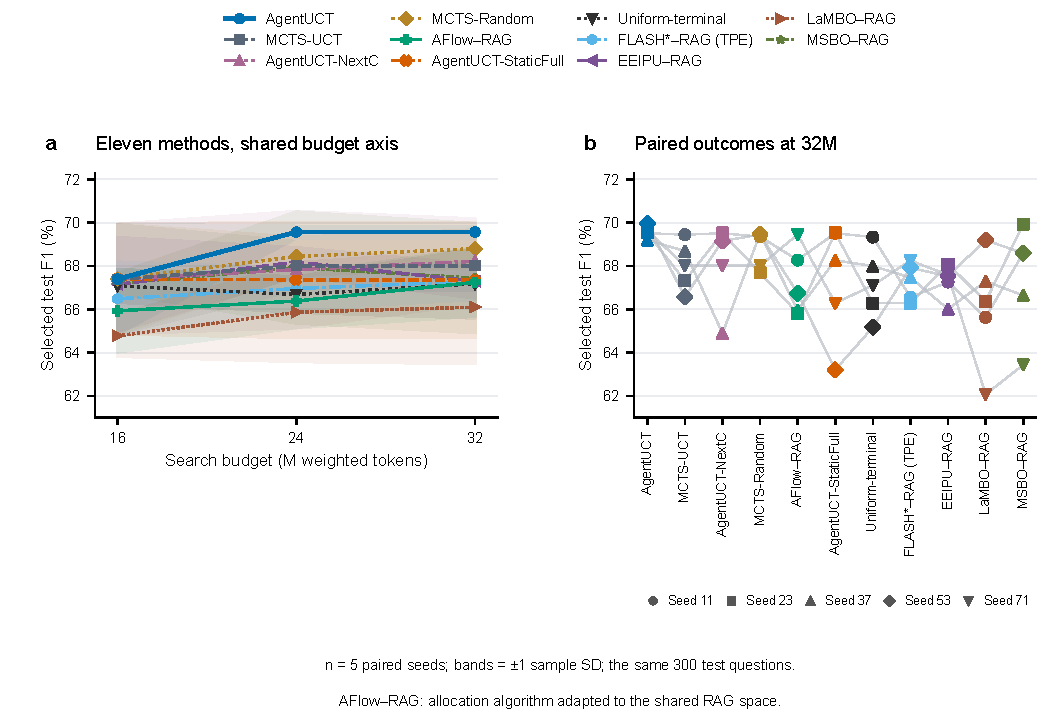
\includegraphics[width=0.96\textwidth]{figures/rag-budget-overlay-20261004/five-seed-budget-overlay.pdf}
\caption{Test F1 after validation selection at actual search-cost cutoffs.
(a) Eleven method means and $\pm$ one sample SD across five paired seeds
share axes. (b) Every paired 32M outcome. Endpoint reuse creates correlated
budget measurements; smaller-budget and seed-level reversals are retained.}
\Description{Eleven methods share test F1 versus actual search budget axes with sample SD bands. A second panel retains all matched seed outcomes at 32 million weighted-token units.}
\label{fig:budget-quality}
\end{figure*}

AgentUCT led AFlow in all seeds at 24M and 32M, and uniform-terminal,
FLASH*, EEIPU and LaMBO in all seeds at 32M. MSBO led in seed 23 by
0.41 points. At 16M, all five sampling/surrogate/stage controls exceeded
AgentUCT in seed 53; LaMBO led by 0.39 points in seed 37 at 24M.
Thus the highest 32M mean is specific to this cohort and does not describe
every seed or budget. Fifty prespecified random workflows reached
$60.58\pm5.22\%$ mean F1 (workflow SD), median $62.11\%$; three fixed
Query2doc--BM25, HyDE--E5 and RankGPT-style adaptations~\citep{sun2023rankgpt} reached 61.60,
62.89 and 62.53\%. All fifty draws, rather than a test-best subset, entered
the reference distribution.

\subsection{Estimator and endpoint-selection ablations}
\label{sec:skip-validation}
AgentUCT's advantage over MCTS-UCT persisted without validation. On the same retained
searches, direct testing of the highest training-F1 workflow gave AgentUCT
$69.24\pm0.74\%$ and MCTS-UCT $67.37\pm0.53\%$ at 32M, with paired
gain $1.87\pm1.24$ points. The supplement retains all sixty training-Top1
method--seed--budget cells. Test outcomes never selected a workflow or
changed a snapshot.

\paragraph{Estimator adaptation.}
\label{sec:static-full-results}
Full suffix pricing exceeded AgentUCT-NextC's mean by 1.73 points at 24M
and 1.35 at 32M; at 32M, three seeds improved and two tied. Direct
training-Top1 selection reduced this gap to 0.35 points. Against
AgentUCT-StaticFull, AgentUCT's paired 32M difference was
$2.21\pm2.89$ points: three gains and two ties, with identical retained
evaluation counts per pair. These interventions support complete-cost
pricing and joint estimator adaptation in this protocol; the static
comparison does not separate cache conditioning, price learning and demand.

Higher F1 did not imply higher full-bill utility. AgentUCT's mean
$C_{\rm opt}$ was 59.003M, compared with MCTS-UCT's 59.624M and
AgentUCT-NextC's 58.319M. Its mean $J$ was 0.03670 above MCTS-UCT and
0.00978 below AgentUCT-NextC, chiefly because of validation cost.
Logical hit rates at 32M were 6.79\% for AgentUCT and 6.81\% for MCTS-UCT.
These paths have different workloads; no matched cache-disabled speedup was
measured. Every saved RAG prefix covered all training queries, placing this
experiment in the exactly compressible full-panel graph case.

\subsection{Generated workflows on GSM8K}
GSM8K~\citep{cobbe2021verifiers} used five paired seeds and panels of 150 training, 300 validation and
300 primary test questions. AgentUCT and MCTS-UCT shared Qwen3.5-4B,
fixed-eight groups, Python operators, proposer/repair settings, counted-error
histories, progressive widening $\min(8,\max(1,\lceil\sqrt N\rceil))$, depth limit
12 and no rollout. They differed in completion pricing. AFlow retained its
Top4 parent policy in the same adaptation. Independent fixed-path cost
calibration froze $C_{\rm ref}=150{,}954.5$ raw tokens and budgets of
6.423M, 12.772M and 19.122M; test quality did not enter calibration.
Up to five training-ranked completed workflows entered validation per snapshot.

\begin{table*}[t]
\centering\small
\caption{Complete GSM8K accuracy (\%), mean $\pm$ sample SD across five
paired seeds at raw-token budgets 6.423/12.772/19.122M. Rows report original
method scores; SD is not a confidence interval.}
\label{tab:generated-complete-main}
\begin{tabular}{llrrr}
\toprule
Task & Method & First & Middle & Largest\\
\midrule
GSM8K & AgentUCT & $93.07\pm1.52$ & $93.00\pm1.49$ & $93.07\pm1.48$\\
 & MCTS-UCT & $92.60\pm1.09$ & $92.60\pm0.86$ & $92.67\pm0.78$\\
 & AFlow & $91.60\pm1.95$ & $92.93\pm1.26$ & $93.07\pm1.40$\\
\bottomrule
\end{tabular}
\end{table*}

At the largest GSM8K cutoff, AgentUCT led MCTS-UCT in three seeds, tied
in one and trailed in one. Its $93.07\%$ mean was exactly equal to AFlow's
before rounding (Table~\ref{tab:generated-complete-main}). Saved traversals
show recursive cost-induced choices; a recorded depth-one choice yielded
zero training score, while AgentUCT seed 71 selected initial node 0 at all
three budgets. Decision evidence therefore does not attribute endpoint
accuracy gains to those particular choices.

The supplement retains all 45 GSM8K quality cells, equally
weighted seed means, sample SDs with denominator $n-1$, and full actual
ledgers. Common questions and repeated endpoints correlate budgets.
Physical failures, candidate errors, repair calls and whole crossing
evaluations remain scored or billed under their original protocols;
overshoot is a subset of the bill, not an extra charge. GSM shared
preparation cost 109,983 raw tokens is a separate one-time item. These raw-token costs remain distinct
from RAG's model-weighted units. Retired proposal-history cohorts and
the earlier bounded pilot do not enter this complete comparison.


\section{Related Work}
UCT backs up adaptive descendant returns~\citep{kocsis2006bandit}; UCB1's
stationary-bandit guarantee~\citep{auer2002finite} does not directly establish
a tree rate. Coquelin and Munos analyze depth-dependent UCT
transients~\citep{coquelin2007bandit}, while Shah et al. use a polynomial bonus
for recursive planning~\citep{shah2020mcts}. Our fixed-table result retains
the logarithmic bonus and derives deficits from actual ancestor backups.

FLASH combines cost-sensitive acquisition and prefix caching
\citep{zhang2016flash}; EEIPU prices memoized prefixes through stage-cost GPs
\citep{essofi2024memoization}; MSBO allocates start/advance decisions using
cascade observations~\citep{torresi2026multistage}. LaMBO optimizes modular
switching costs relative to the preceding configuration~\citep{lin2021lambo}.
AgentUCT restores prefixes from any earlier evaluation and allocates using
complete terminal returns. AFlow edits generated programs using execution
feedback and mixed parent selection~\citep{zhang2024aflow}. Our adapters
compare these whole policies within shared systems. Metareasoning motivates
evaluating the final decision alongside computation cost~\citep{hay2012selecting}.

\section{Discussion and Conclusion}
Completion pricing improved selected-workflow F1 in HotpotQA with similar
numbers of completed evaluations to MCTS-UCT. The advantage under direct
training-Top1 testing supports an allocation effect that does not require
post-search validation. Saved choices locate this evidence at the root.
GSM8K records recursive cost-induced decisions, but those traces do not
identify the contribution of individual choices to test accuracy.

The estimator's scope matters. Full suffix pricing improved quality over
AgentUCT-NextC while its validation bill lowered auxiliary full-bill utility.
The static ablation tests cache conditioning, price learning and continuation
adaptation jointly; its three wins and two ties do not separate their causal
contributions. Shared execution reuse is available to all methods. The
full-panel RAG graph admits exact prefix aggregation, so these experiments
do not demonstrate a gain from a finer graph representation or a no-cache
speedup.

The GSM8K comparison has a small mean gain over MCTS-UCT and an exact
mean tie with AFlow at the largest budget. Completion prices are a useful
allocation signal in the measured RAG regime; this generated-program
comparison does not establish broad task transfer. The theorem explains persistence of quality exploration
under finite cold execution. It leaves practical forecast calibration,
recurring-cost guarantees and finite-budget test optimality open.
